在避免死锁的办法中,所施加的限制条件较弱,有可能获得较好的系统性能。在该方法中把系统的状态分为安全状态和不安全状态,\textbf{只要能使系统始终处于安全状态,便可以避免死锁的发生}。

\textbf{{1.安全状态与不安全状态}}\\

安全状态:按某方案分配资源系统一定不会进入死锁。

不安全状态:按某方案分配资源,系统{有可能}进入死锁。

{\textbf{安全状态一定不会导致死锁,不安全状态不一定会导致死锁,但是有可能导致死锁}}。

\textbf{{2.银行家算法}}

银行家算法中使用的数据结构如下:

a. 可利用资源向量Available;

b. 最大需求矩阵Max;

c. 分配矩阵Allocation;

d. 需求矩阵Need。

\textbf{``矩阵三兄弟''具有如下关系:}Need{[}i{]}{[}j{]}=Max{[}i{]}{[}j{]}-Allocation{[}i{]}{[}j{]};

银行家算法的流程图如下:

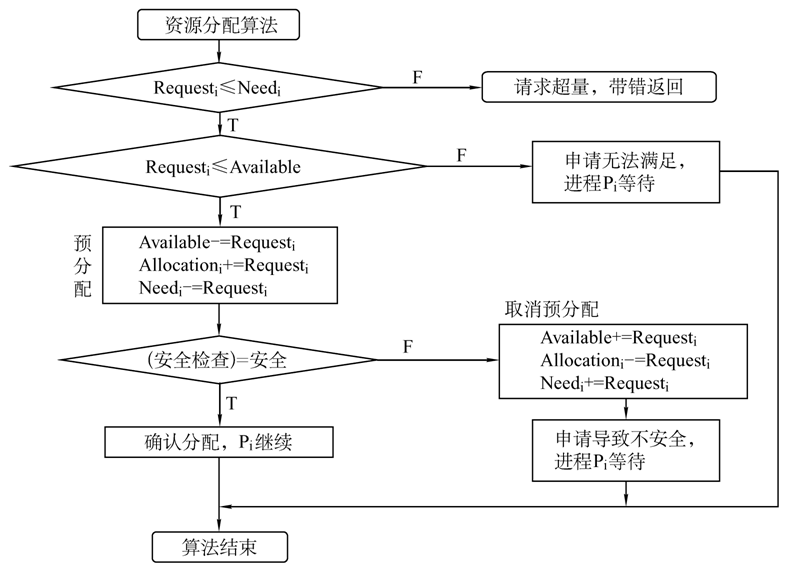
\includegraphics[width=3.33333in,height=2.41667in]{png-jpeg-pics/EA9C2698F88D504B5EE6D4F328CD9C0C.png}
